\chapter{Modellierung und Entwurf}
\label{cha:Modellierung und Entwurf}

In diesem Kapitel werden die funktionalen Anforderungen aus dem Abschnitt \ref{sec:anforderungsdefinition} spezifiziert. Modelle für die einzelnen funktionalen Anforderungen sollen entwickelt werden. Die Modelle veranschaulichen das geforderte funktionale Verhalten der Software. Voraussetzung für die Entwicklung der Modelle ist die Konkretisierung der funktionalen Anforderungen. Diese Konkretisierung beinhaltet die Festlegung der Bestandteile die für eine Implementierung der funktionalen Anforderung benötigt werden. Ziel des Kapitels ist es, die wichtigsten Bestandteile einer funktionalen Anwendung herauszubilden, dieses Bestandteile zu definieren und zu veranschaulichen. 



\section{Tic Tac Toe}
\label{sec:Tic Tac Toe}

Tic Tac Toe ist ein Spiel, welches mit genau zwei Spielern gespielt wird. Während eines gesamten Spiels darf ein Spieler nur Kreuze setzen und der andere Spieler nur Kreise. Ein Spieler der während einer Partie nur Kreuze setzen darf wird als Kreuzspieler und sein Gegner als Kreisspieler bezeichnet. Wir können uns die Kreuze und Kreise als Spielsteine vorstellen, die sobald sie auf das Spielfeld gesetzt wurden, nicht mehr verändert oder verschoben werden können. Das Spielbrett ist eine 4 x 4 große Matrix, also können maximal 16 Spielsteine in diese Matrix gesetzt werden. Der Kreuzspieler muss immer als erster beginnen. Im ersten Spielzug stehen dem Kreuzspieler 16 mögliche Positionen zur Verfügung. Die Anzahl der möglichen Positionen reduziert sich jede Runde um 1, weil jede Runde genau ein gesetzter Spielstein ein Spielfeld besetzt. Folglich ist die maximale Länge einer Spielzugsequenz bei einem 4 x 4 Spielfeld gleich 16. Es ist auch möglich, dass das Spiel bereits vor der 16. Runde beendet wird. \\

\paragraph{Spielzüge} jeder Spieler setzt abwechselnd entweder ein Kreuz oder einen Kreis in ein Spielfeld des Spielbretts. Ein Spielstein kann in jedes der 16 Spielfelder gesetzt werden, außer dieses ist bereits mit einem anderen Spielstein besetzt, dann muss der Spieler ein anderes Spielfeld auswählen. Die Spieler führen solange Ihre Spielzüge aus, bis eine Siegesformation eines Spielsteintyps erreicht ist oder alle Spielfelder besetzt sind. 

\paragraph{Ziel des Spiels} ist es vier Kreuze oder vier Kreise in einer bestimmten Position anzuordnen. Es existieren mehrere unterschiedliche Anordnungen von Spielsteinen, die das Spiel beenden und einen Sieg herbeiführen. Bei einem 4 x 4 Spielfeld existieren vier vertikale, vier horizontale und zwei diagonale Anordnungen der Spielfiguren, welche einen Sieg herbeiführen würden. Insgesamt zehn verschiedene Siegesanordnungen für beide Spieler. Sind alle Spielfelder besetzt und für keinen der Spieler ist eine Siegesformation aufgetreten, dann gewinnt beziehungsweise verliert keiner der beiden Spieler und es entsteht ein Unentschieden. Gewinnt ein Spieler mit einer Siegesanordnung seiner Spielsteine, dann verliert der andere Spieler dadurch automatisch in gleicher Höhe (Nullsummenspiel). \\

\begin{figure}[!htbp]
  \centering
  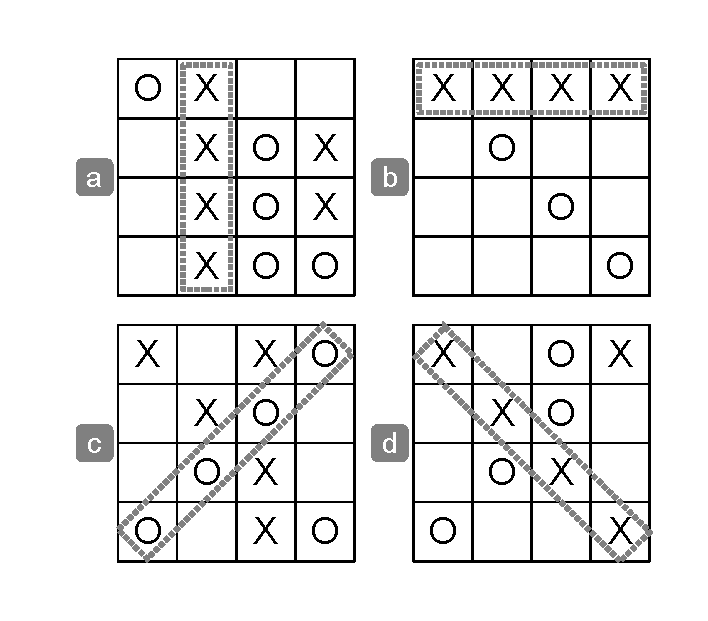
\includegraphics[scale = 1]{inhalt/abbildungen/siegesbedingungen_tictactoe.pdf}
  \caption{Veranschaulichung der vertikalen (a), horizontalen (b) und diagonalen (c, d) Siegesbedingung.}
  \label{fig:siegesbedingungen_tictactoe}
\end{figure}

Vier mögliche Siegesformationen sind in Abbildung \ref{fig:siegesbedingungen_tictactoe} dargestellt. (a) Der Kreuzspieler gewinnt knapp gegen seinen Kontrahenten mit einer ununterbrochenen vertikalen Anordnung seiner Spielsteine. Der Kreisspieler hätte fast eine diagonale Reihe aus Kreisen verbunden, diese wurde jedoch vom Kreuzspieler mit einem Spielstein unterbrochen. Zudem hätte der Kreisspieler auch fast eine vertikale Reihe ohne Unterbrechungen vervollständigt, aber der Sieg des Kreuzspielers hat die Partie vorher beendet. (b) Der Kreuzspieler erreicht eine horizontale Siegesanordnung, vier Kreuzsteine in einer horizontalen Zeile angeordnet. (c) Der Kreisspieler besiegt den Kreuzspieler mit einer diagonalen Siegesanordnung. (d) Der Kreuzspieler gewinnt ebenfalls durch eine diagonale Siegesformation seiner Spielsteine. 

\subsection{Lernen mit Strategieverbesserung}
Die nachfolgend aufgestellte Strategie ist keine optimale Strategie, das heißt es ist nicht möglich mit dieser Strategie immer zu gewinnen oder mindestens ein Unentschieden zu erreichen. Das Ziel des Lernverfahrens ist es, diese nicht optimale Strategie in eine optimale Strategie oder zumindest eine annähernd optimale Strategie zu transformieren. Eine optimale Strategie würde gegen unaufmerksame oder unerfahrene Gegner verhältnismäßig oft Gewinnen und nicht gegen diese Verlieren, Unentschieden können trotzdem vorkommen. Ist der Gegner ein perfekter TicTacToe Algorithmus oder ein TicTacToe Großmeister, dann sollte die optimale Strategie überwiegend Unentschieden hervorbringen. Eine optimale Strategie sollte in 100 Spielen gegen einen Großmeister oder eine andere optimale Strategie (dieselbe optimale Strategie oder möglicherweise eine andere) 100 Unentschieden erringen. Siege sind theoretisch höherwertiger als Unentschieden, aber innerhalb der TicTacToe Spielwelt sind diese gegen einen Großmeister oder einen perfekten Algorithmus äußerst unwahrscheinlich. \\

Unser Lernalgorithmus oder im Kontext des verstärkenden Lernens unser Agent, erhält eine Belohnung von +1 wenn er eine Party (eine komplette Spielzugsequenz bis ein Spielergebnis feststeht) TicTacToe gewinnt. Verliert er eine Party, dann wird er bestraft mit dem numerischen Wert -1. Bei einem Unentschieden wird der Agent ebenfalls belohnt, aber die Belohnung ist nicht so hoch wie bei einem Sieg, denn wir wollen das Verhalten des Lernverfahrens so trainieren, dass es eher einen Sieg erlangen wird als ein Unentschieden, aber auf jeden Fall eine Niederlage vermeidet. Der Agent soll immer versuchen diesen nummerischen Wert zu maximieren, darum wird er eine Niederlage vermeiden. Der Agenten könnte auch so trainiert werden, dass er immer absichtlich verlieren würde, dafür müsste jeder, vom Agenten ausgeführte, Spielzug (egal welcher Spielzug) eine hohe negative nummerische Bestrafung hervorbringen. Das Ziel des Agenten wäre dann, schnellstmöglich ein Ende des Spiels zu provozieren und weil verlieren sicherer und kürzer ist als gewinnen oder ein Unentschieden, würde der Agent lernen absichtlich zu verlieren. Interessant wäre das Spielergebnis, wenn zwei Agenten gegeneinander antreten würden, die immer schnellstmöglich verlieren wollen, dann entstünden theoretisch ausschließlich Unentschieden.


\myparagraph{Kombination von überwachtem und verstärkenden Lernen}
Dem Lernverfahren eine Strategie vorzugeben, welche für jeden Zustand festlegt welche Aktion ausgeführt werden soll, ähnelt stark dem überwachten Lernen. Bei einem überwachten Lernverfahren würde der Agent eine Liste von Zuständen und Aktionen als Eingabeparameter bekommen, in dieser Liste sind den Zuständen Aktion zugeordnet. Der Agent lernt die Liste von Zustand-Aktions-Paaren und dadurch lernt er, bei welcher Spielfiguren Anordnung (Zustand), welche Position mit seiner Spielfigur belegt werden sollte (Aktion). Die Zustände wären in diesem Trainingsset Eigenschaften (Features) und die Aktionen wären Zielvariablen (Target Values). In der Theorie wird überwachtes Lernen mit verstärkendem Lernen kombiniert, um ein schnell konvergierendes Lernverfahren zu erhalten. Die Konvergenz bezieht sich auf die Strategie, welche das Lernverfahren optimieren soll. Der Agent versucht diese nicht optimale Strategie schrittweise in eine optimale Strategie umzuwandeln und wenn ihm dies gelingt, dann hat die verbesserte nicht optimale Strategie eine Konvergenz mit der optimalen Strategie erreicht, dass bedeutet die Ausgangsstrategie wurde zu einer optimale Strategie weiterentwickelt. \\

Warum eigentlich kein reines überwachtes oder verstärkendes Verfahren? Eine optimale Strategie nur durch überwachtes Lernen zu erstellen, würde ein Trainingsset voraussetzen, indem jeder Zustand der Spielwelt erfasst ist und jeder dieser Zustände müsste genau eine optimale Aktion abbilden. Bei komplexeren Probleme kann das sehr hohe Kosten verursachen oder es ist überhaupt nicht möglich, denn für viele Zustände ist die optimale Aktion nicht bekannt. Das vier mal vier TicTacToe ist noch ein recht simpler Vertreter der Strategiespiele und soll dazu dienen, die Anwendung und Modellierung der Lernverfahren und der Strategien zu veranschaulichen. Ob ein Strategiespiel im Kontext der Lernverfahren simpler oder komplexer ist ,hängt von seinen Zustands- und Aktionsdimensionen ab. Die Größe das Spielfelds, die Anzahl verschiedener Aktionen pro Spielsituation und die durchschnittliche Anzahl der Spielzüge, entscheiden über die Komplexität des Strategiespiels. Wenn das überwachte Lernen einer optimalen Strategie aufgrund größerer Dimensionen nicht möglich ist, können wir dann nicht ein verstärkendes Lernverfahren implementieren? \\

Unterabschnitt \ref{subsec:Lernen ohne Strategie} behandelt die Thematik des reinen verstärkenden Lernens. Daher werden die Vor- und Nachteile des reinen verstärkenden Lernens jetzt nicht weiter analysiert. Wir konzentrieren uns in diesem Abschnitt darauf, welche Strategien entwickelt, wie diese Strategien praktisch angewendet und wie die angewendeten Strategien optimiert werden können. Bei der Entwicklung der Strategie muss besonders darauf geachtet werden, worauf der Agent aufmerksam gemacht werden soll. Unter Umständen ist es besonders Wahrscheinlich zu gewinnen, wenn eine besondere Spielstellung erreicht wurde oder  einzelne Spielfelder erleichtern einen Sieg und sollten daher eher besetzt werden als andere möglicherweise unwichtigerer Spielfelder. Die Ausgangsstrategie ist also ein wichtiger Faktor für die Konvergenz-Geschwindigkeit.

\myparagraph{Das Spielfeld}

\begin{figure}[!htbp]
  \centering
  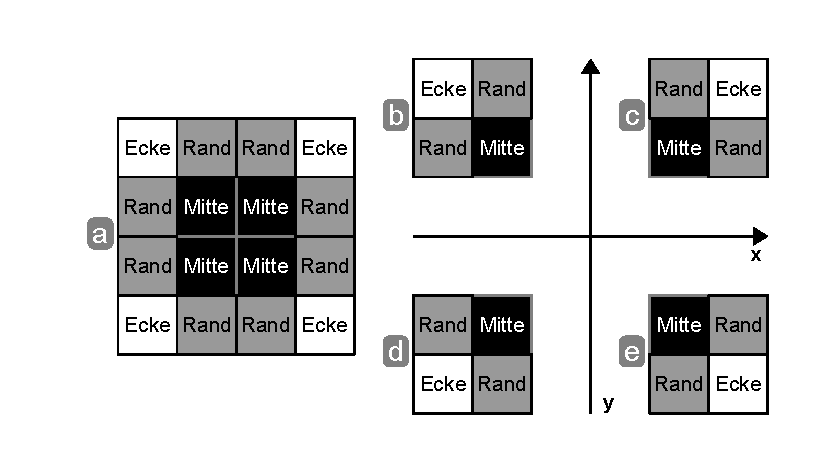
\includegraphics[scale = 1]{inhalt/abbildungen/symmetrie_tictactoe_spielfeld.pdf}
  \caption{Symmetrie Eigenschaften des vier mal vier Tic Tac Toe Spielfelds.}
  \label{fig:symmetrie_tictactoe_spielfeld}
\end{figure}

Um eine Strategie zu entwickeln werden wir uns zuerst das Spielfeld ansehen und dieses analysieren. Das vier mal vier TicTacToe Spielfeld hat 16 Spielfelder, vier Eckfeldern, vier Mittelfeldern und acht Randfeldern (siehe Abbildung \ref{fig:symmetrie_tictactoe_spielfeld} a). Ziehen wir eine horizontale und eine vertikale Achse durch das Spielfeld, dann sind bestimmte Symmetrieeigenschaften zu erkennen, Abbildung \ref{fig:symmetrie_tictactoe_spielfeld} zeigt b und c, sowie d und e sind symmetrisch zur y-Achse, b und d, sowie c und e sind symmetrisch zur x-Achse und b und e, sowie d und c sind symmetrisch, wenn man sie an der x-Achse und der y-Achse spiegelt. Diese Symmetrieeigenschaften sind wichtig für die Reduktion der Strategien, das heißt wenn eine Strategie auf b angewendet werden kann, dann auch auf c, d und e.

\myparagraph{Kontrolliere die Mitte}

Um über bestimmte Spielfelder reden zu können, müssen wir eine konkrete Identifikation der einzelnen Spielfelder vornehmen. In Abbildung \ref{fig:tictactoe_spielfeld_indizes} wird daher jedem der Spielfelder ein Index zugewiesen.

\begin{figure}[!htbp]
  \centering
  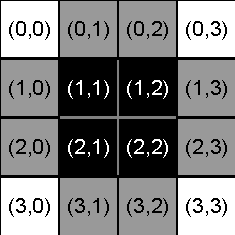
\includegraphics[scale = 1]{inhalt/abbildungen/tictactoe_spielfeld_indizes.pdf}
  \caption{Die Indizes der einzelnen Spielfelder.}
  \label{fig:tictactoe_spielfeld_indizes}
\end{figure}

Die Eröffnungsstrategie konzentriert sich auf die Kontrolle der Mittelfelder. Hat der Agent beziehungsweise das Lernverfahren das Recht auf den ersten Zug befindet er sich immer in Zustand $s_0$. In diesem Zustand sind alle Spielfelder leer und der Agent kann durch Zufall eines der vier mittleren Felder wählen. Der Agent trifft diese Entscheidung zufällig, weil zu diesem Zeitpunkt und in diesem Zustand alle vier Mittelfelder die gleiche positive numerische Belohnung erbringen (siehe Abbildung \ref{fig:kontrolliere_die_mitte} 1). Die Rand- und Eckfelder haben keine numerische Belohnung, aber auch keine numerische Bestrafung für den Agenten, so wird sichergestellt, dass das Lernverfahren sich für ein mittleres Spielfeld entscheidet. Nachdem der gegnerische Spieler seine Spielfigur gesetzt hat, soll der Agent die zweite Spielfigur ebenfalls auf ein mittleres Feld setzen, jedoch eher auf ein mittleres Spielfeld, welches sich in einer Reihe ohne eine gegnerische Spielfigur befindet. \\

\begin{figure}[!htbp]
  \centering
  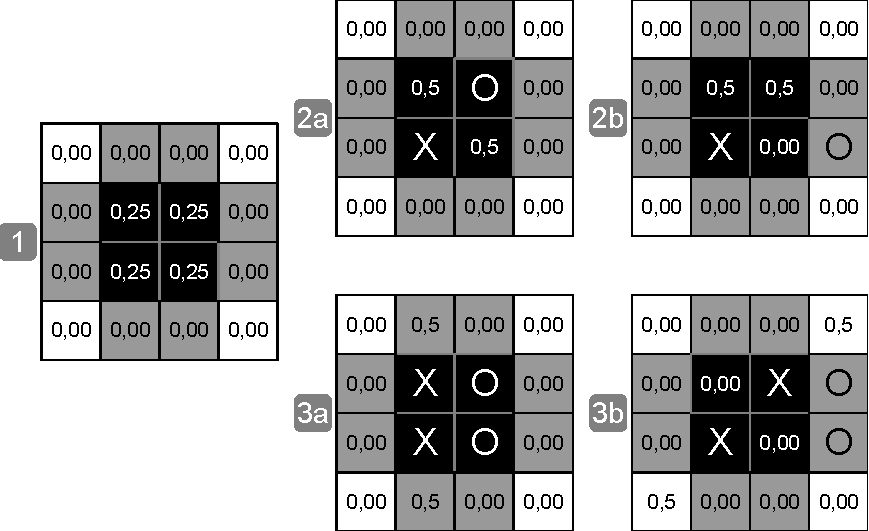
\includegraphics[scale = 0.8]{inhalt/abbildungen/kontrolliere_die_mitte.pdf}
  \caption{Strategie um die Mitte zu kontrollieren.}
  \label{fig:kontrolliere_die_mitte}
\end{figure}

Von jetzt an betrachten wir die beiden Kontrahenten Alice (Spielfiguren X) und Bob (Spielfiguren O) als zwei Instanzen des selben Lernverfahrens, dass heißt der Agent spielt gegen einen anderen Agenten mit exakt dem selben Verhalten.
In Abbildung \ref{fig:kontrolliere_die_mitte} (2a) setzt Alice ihre Spielfigur auf das Feld (2,1) und Bob auf (1,2). Die Strategie der Mittelfeld Kontrolle offenbart unserer Agentin Alice zwei Aktionsmöglichkeiten mit positiver Belohnung. Setzt Agentin Alice ihre Spielfigur auf die Mittelfelder (1,1) oder (2,2), dann erhält sie einen numerische Belohnung von +0,5. Alice entscheidet durch Zufall welches der beiden Felder mit der gleichgroßen größtmöglichen Belohnung sie auswählt. Alice entscheidet sich durch Zufall für das Spielfeld (1,1) und Bob, der ebenfalls der Strategie der Mittelfeld Kontrolle folgt, entscheidet sich für das letzte nicht besetzte Mittelfeld (Abbildung \ref{fig:kontrolliere_die_mitte} 3a).\\

Sollte Agent Bob eine andere gelernte Strategie verfolgen und zum Beispiel ein Randfeld besetzen, dann werden Agentin Alice andere Aktionen von ihrer Strategie Vorgeschlagen. In einem alternativen Spielverlauf (Abbildung \ref{fig:kontrolliere_die_mitte} 2b) setzt Agent Bob seine Spielfigur nicht auf das Spielfeld (1,2), sondern auf das Spielfeld (2,3). Die Strategie der Kontrolle der Mittelfelder bevorzugt Mittelfelder, die in einer leeren vertikalen, horizontalen oder diagonalen Reihe sind, bezogen auf die bereits gesetzte Spielfigur. Das Mittelfeld (2,2) wird uninteressant für die Strategie von Alice, weil eine mögliche horizontale Reihe aus vier gleichen Spielsteinen bereits nicht mehr möglich ist. Dahingegen schlägt die Strategie die Mittelfelder (1,1) und (1,2) mit einer numerischen Belohnung von +0,5 vor. Setzt Alice ihre Spielfigur auf das Mittelfeld (1,1), dann ist eine vertikale Verbindung von vier gleichen Spielfiguren möglich und setzt Alice ihre Spielfigur auf das Mittelfeld (1,2), dann ist eine diagonale Verbindung von vier gleichen Spielfiguren möglich. \\

Agentin Alice entschiedet durch Zufall ihre Spielfigur auf das Mittelfeld (1,2) zu setzen, denn der Agent soll durch Zufall entscheiden, wenn für mehrere Aktionen in einem Zustand die gleich Hohe größtmögliche Belohnung vergeben wird. Agent Bob setzt daraufhin seine Spielfigur auf das Randfeld (1,3). Ein neue Spielsituation (Zustand) entsteht (Abbildung \ref{fig:kontrolliere_die_mitte} 3b). Alice erhält von der Strategie der Mittelfeld Kontrolle die Aktionsoptionen (0,3) und (3,0). Beide Aktionsoptionen werden mit +0,5 belohnt. Diese Strategie berücksichtigt nicht, dass Agent Bob bereits zwei Spielsteine in einer ungestörten vertikalen Verbindung positioniert hat. Daher kann Alice durch Zufall entscheiden welche Aktion sie ausführt. Eine bessere Strategie würde Alice in diesem Zustand diese Option nicht lassen, denn das Eckfeld (0,3) ist in dieser Spielsituation attraktiver als das Eckfeld (3,0). Eckfeld (0,3) erweitert die diagonale ungestörte Verbindung von Agentin Alice auf eine Länge von drei und gleichzeitig würde die vertikale ungestörte Verbindung von Agent Bob gestört werden. Eine optimale Strategie würde Alice mit einer Belohnung von +0,75 das Eckfeld (0,3) empfehlen. \\ 

Bevor wir Alice und Bob die Möglichkeit geben die Strategie selber zu verbessern beziehungsweise eigenständig zu entwickeln und solche Auffälligkeiten und Muster in die Strategie zu integrieren, werden wir die Ausgangsstrategie noch um eine Teilstrategie erweitern. \\

\myparagraph{Verteidigung ist der beste Angriff}

Diese Strategie konzentriert sich darauf, gegnerische Stellungen zu erkennen und dahingehend Gengenmaßnahmen einzuleiten. Abbildung \ref{fig:verteidigung_ist_angriff} verdeutlicht gefährliche Spielsituationen, in denen die Strategie Gegenmaßnahmen vorschlagen sollte. Horizontale Verbindugsmöglichkeiten (1a - 1d) 

\begin{figure}[!htbp]
  \centering
  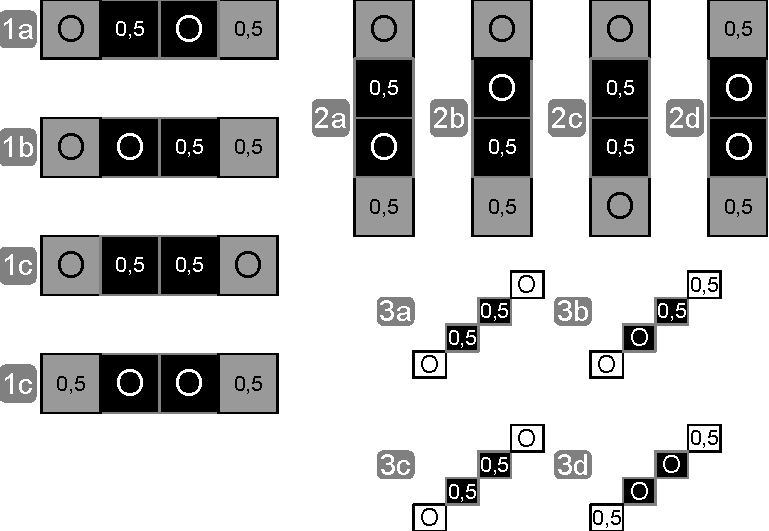
\includegraphics[scale = 0.8]{inhalt/abbildungen/verteidigung_ist_angriff.pdf}
  \caption{TicTacToe Angriffsstrategien (aus der Sicht von Bob) und Verteidigungsstrategien (aus der Sicht von Alice).}
  \label{fig:verteidigung_ist_angriff}
\end{figure}

\subsection{Lernen ohne Strategie}
\label{subsec:Lernen ohne Strategie}

\section{Reversi}
Das Spiel Reversi oder auch Othello genant, wird auf einem 8x8 Spielbrett gespielt. Es ist ein Spiel für zwei Personen die gegeneinander antreten. Eine Person setzt weiße runde Spielsteine und die andere Person schwarze runde Spielsteine. Jede neue Partie Reversie beginnt im selben Ausgangszustand (siehe Abbildung \ref{fig:ausgangssituation_reversi}). Die Spieler setzen nacheinander in ihren Spielzügen genau einen Spielstein. Wie beim klassischen Tic Tac Toe aus Abschnitt \ref{sec:Tic Tac Toe} behalten die Spieler während des gesamten Spiels ihre Spielsteinfarbe und einmal gesetzte Spielsteine können ihre Position nicht mehr verändern. \\

\begin{figure}[!htbp]
  \centering
  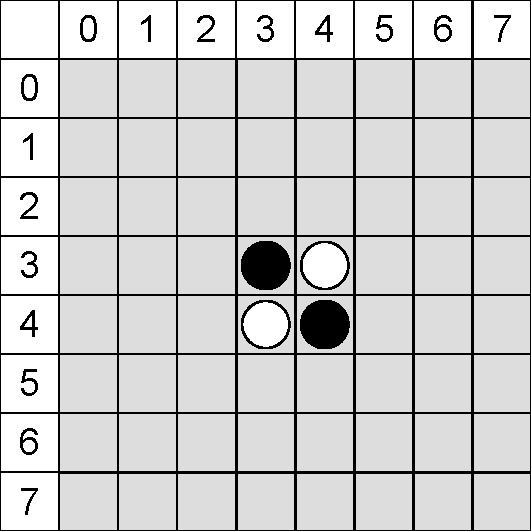
\includegraphics[scale=0.5]{inhalt/abbildungen/ausgangssituation_reversi.pdf}
  \caption{Ausgangssituation einer beginnenden Partie Reversi. Die äußeren weiß hinterlegten Reihen in denen sich Zahlen befinden, dienen dazu die Positionen der einzelnen Spielfelder genau zu definieren. In der Ausgangsspielsituation befinden sich bereits 2 weiße Spielsteine an den Positionen (3,4) und (4,3) und zwei schwarze Spielsteine an den Positionen (3,3) und (4,4).}
  \label{fig:ausgangssituation_reversi}
\end{figure}

Eine Besonderheit von Reversi ist, dass gesetzte Spielsteine ihre Farbe ändern können. Werden z.B. zwei weiße Spielsteine von zwei schwarzen in einer horizontalen Linie eingeschlossen, dann werden die weißen Spielsteine in schwarze umgewandelt beziehungsweise umgedreht. Das erobern der gegnerischen Spielsteine ist vom aktuell gesetzten Spielstein abhängig. Die Siegesbedingung von Reversi ist es, am Ende des Spiels, mehr Spielsteine seiner eigenen Farbe zu haben als der Gegner Spielsteine in seiner Farbe hat. Das Spiel endet, wenn keiner der beiden Spieler mehr einen Spielstein, nach den Regeln des Spiels, auf das Spielbrett setzen kann. \\

\paragraph{Spielzüge} sind bei Reversi nicht beliebig, sie unterliegen bestimmten Regellungen. Eine Regel für das Setzen eines Spielsteins ist, nur wenn mindestens ein gegnerischer Spielstein erobert wird, darf ein Spielstein an diese Stelle gesetzt werden. Weiterhin  darf ein Spielstein nur dann gesetzt werden wenn, ein anderer Spielstein(Anker), mit der gleichen Farbe, in einer diagonalen, vertikalen oder horizontalen Linie, existiert. Es dürfen auch keine freien Felder zwischen dem zu setzendem Stein und dem Anker liegen. Ein Anker ist ein Spielstein mit der selben Farbe wie der zu setzende Spielstein. Ein zu setzender Spielstein kann mehrere Anker haben, aber er muss mindestens einen und kann maximal acht Anker haben.\\

Der Anker in Abbildung \ref{fig:zuege_schwarz_reversi} ist der schwarze Spielstein an der Stelle (3,3). (a) In diesem Beispiel soll schwarz am Zug sein und einen Spielstein platzieren. Die Positionen (3,1) und (3,6) ermöglichen eine horizontale, (5,3) ermöglicht eine vertikale und (5,1), (0,6) und (7,7) ermöglichen eine diagonale Verbindung mit dem Anker auf Position (3,3). Die meisten gegnerischen Spielsteine könnte schwarz erobern, indem er seinen Spielstein auf das Spielfeld (7,7) setzt. (b) Setzt der Spieler seinen schwarzen Spielstein an die Position (3,1), dann hat dieser 3 Anker. Einen vertikalen Anker (0,1), einen horizontalen Anker (3,3) und einen diagonalen Anker (0,4). Insgesamt würden 5 weiße Spielsteine erobert werden, also 2 mehr als in (a) maximal möglich wären. \\

\begin{figure}[!htbp]
  \centering
  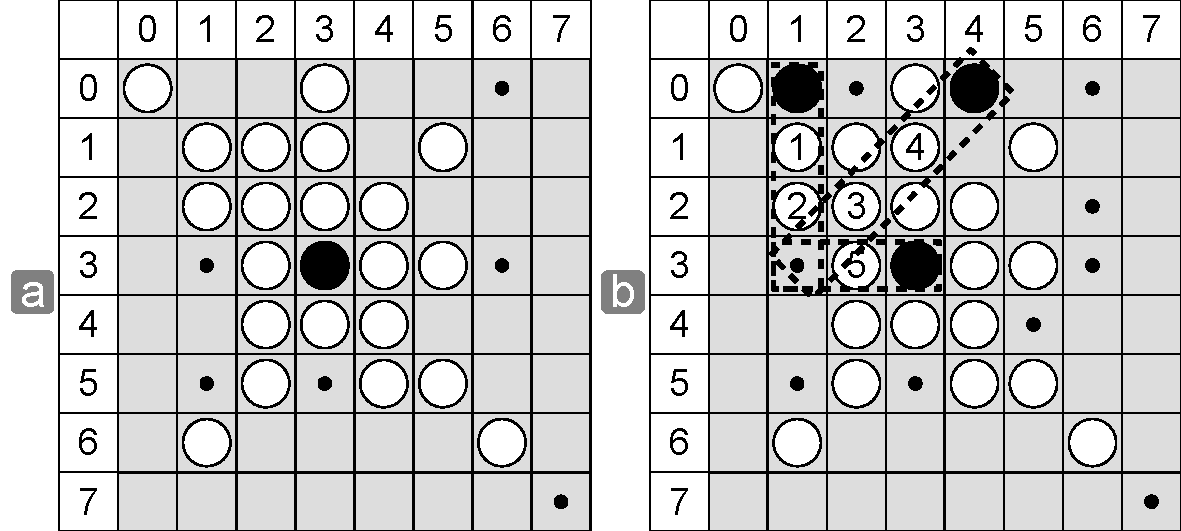
\includegraphics[scale=0.5]{inhalt/abbildungen/zuege_schwarz_reversi.pdf}
  \caption{Zwei möglicherweise nicht in der Praxis auftretende Spielsituationen, die einzig verdeutlichen sollen welche Zugmöglichkeiten der Spieler mit den schwarzen Spielsteinen hat und warum nur diese Züge möglich sind. Die kleinen schwarzen Punkte zeigen die Positionen an denen ein schwarzer Spielstein gesetzt werden darf. (a) Eine Spielsituation mit maximal einem möglichen Anker. (b) Eine Spielsituation mit maximal 3 möglichen Ankern für die Position (3,1).}
  \label{fig:zuege_schwarz_reversi}
\end{figure}


\section{Tic Tac Toe Heuristik}
\label{sec:Tic Tac Toe Heuristik}

\section{Reversi Heuristik}
\label{sec:Reversi Heuristik}

\section{Die Strategiespielumgebungen Tic Tac Toe und Reversi}

\myparagraph{getPossibleActions()}
Berechnen eine Liste von Positionskoordinaten in der Form: 

\begin{equation*}
[Tupel(X_a Koordinate, Y_b Koordinate), ...].
\end{equation*}

Diese Koordinaten geben die Spielfelder an, welche in einem korrekten Spielzug, von dem aktuellen Spieler, belegt werden können. Aus dieser Liste von Aktionen wählt der Spieler oder der Agent eine mögliche Aktion aus.\\

\section{Agent des Zufalls}
Der Agent des Zufalls ist der womöglich schlechteste Spieler. Seine Entscheidungen werden durch Suchverfahren, Heuristiken oder Lernverfahren beeinflusst. Theoretisch sollte dieser Agent im Vergleich zu den anderen Agenten am meisten verlieren und am wenigsten gewinnen, denn er wird Strategielos eine zufällige Aktion aus einer Menge von möglichen Aktionen in einem Spielzustand auswählen. Die Menge von möglichen Aktionen wird von den Spielumgebungen Tic Tac Toe und Reversi bereitgestellt (siehe Funktion getPossibleActions()). Der Zufallsagent selbst benötigt lediglich eine Funktion:\\

\myparagraph{getRandomAction(possibleActionList).}
Diese Funktion erhält eine Liste von möglichen Aktionen und liefert eine zufällig ausgewählte Aktion aus dieser Liste zurück.

\section{Agent ohne Lernen}
Der Agent ohne Lernen bedient sich diverser Spieltheoretischer Verfahren aus dem Grundlagenkapitel \ref{sec:Spiele mit Gegner} Spiele mit Gegner. Auf der Basis des alpha-beta gekürzten Minimax Suchbaumverfahrens versucht der Agent bis zu einer festgelegten Suchtiefe ein optimales Ergebnis zu finden. Die festgelegte Suchtiefe wurde aus dem Abschnitt \ref{subsec:Iterativ vertiefende Tiefensuche} Iterativ vertiefende Tiefensuche in den Algorithmus des nicht lernenden Agenten übernommen. Diese maximale Suchtiefe begrenzt die Rechenzeit des Agenten, sodass der Agent beim explorieren und expandieren des Suchbaums irgendwann abbricht und das bisher beste gefundene Ergebnis zurück gibt. \\

Diese Rechenzeitverbesserung ist nur durch die Verwendung einer Heuristik möglich. Wie bereits in Abschnitt \ref{subsec:Heuristik} Heuristik erklärt, ermöglicht es die Heuristik oder Bewertungsfunktion auch nicht Blattknoten des Suchbaums zu evaluieren, sprich den Nutzen von nicht Endzuständen und Endzuständen zu berechnen. Die Qualität der Heuristik ist ausschlaggebend für die Qualität (Spielstärke) dieses nicht lernenden Agenten. Der nicht lernende Agent hat keine Möglichkeit diese Heuristik anzupassen. Dahingegen kann der Agent mit TD-Lernen die Parameter der Ausgangsheuristik, anhand seiner Spielerfahrung, anpassen. Der Agent ohne Lernen bietet folgende Funktionalitäten:

\myparagraph{getStrategicTicTacToeAction(ticTacToeGameState)}
Der Input dieser Funktion ist ein Tic Tac Toe Objekt, welches den aktuellen Spielstatus repräsentiert. Wie bereits erklärt sucht diese Funktion mittels Alpha-Beta-Suche bis zu einer begrenzten Suchtiefe nach dem bestmöglichen Zustandsnutzen. Dieser Zustandsnutzen wird durch die in Abschnitt \ref{sec:Tic Tac Toe Heuristik} entworfene Tic Tac Toe Heuristik berechnet. Der zurückgegebene Wert ist die Aktion, welche die erste Aktion des Pfades (Aktionssequenz) zum gefundenen bestmöglichen Zustandsnutzen ist.  

\myparagraph{getStrategicReversiAction(reversiGameState)}
Diese Funktion ist der Funktion getStrategicTicTacToeAction(ticTacToeGameState) sehr ähnlich, nur dass diese auf die Reversi Strategiespielwelt angewendet wird. Der Input der Funktion ist somit ein Reversi Objekt und die verwendete Heuristik ist ebenfalls auf Reversi zugeschnitten(siehe Abschnitt \ref{sec:Reversi Heuristik}). Der Output ist die vorgeschlagene bestmögliche Aktion, im aktuellen Spielzustand, hinsichtlich der abgeschnittenen Suche und der Reversi Bewertungsfunktion.

\paragraph{Alternative Realisierung} wäre z.B. die Aufteilung des Agenten ohne Lernen in zwei Agentenklassen. Ein Agent für Tic Tac Toe und ein Agent für Reversi. Beide Agenten ohne Lernen würden dann über eine Funktion getStrategicAction(gameState) verfügen. Eine andere alternative wäre die Übergabe der Heuristiken an die Funktionen. In einer Programmiersprache in der Funktionen einer höheren Ordnung (Higher-order functions) erlaubt sind, könnten die Heuristiken für Reversi und Tic Tac Toe als Eingabeparameter übergeben werden. Auf diese Weise müsste nur ein nicht lernender Agent und eine Funktion getStrategicAction(gameState, heuristicFunction) implementiert werden. Wir wollen die funktionale Programmierung in dieser Arbeit jedoch nicht anwenden, sondern nur eine mögliche alternative Implementierung aufzeigen. Diese beiden alternativen Realisierungen können auch auf die lernenden Agentenmodelle übertragen werden.

\section{Agent mit TD-Lernen}
Die Aufgabe des Agenten mit TD-Lernen ist, dass verbessern einer gegebenen Heuristik. Unter Verwendung dieser möglicherweise verbesserten Heuristik, soll der Agent eine möglichst optimale Aktion auswählen. Der Agent verbessert die Bewertungsfunktion durch Aktualisierung bzw. Anpassung der Parameter $\theta = \theta_1, ... \theta_n$. 

\begin{equation*}
\hat{U}_\theta(s) = \theta_1 f_1(s) + \theta_2 f_2(s) + ... + \theta_n f_n(s)
\end{equation*}



\section{Agent mit Q-Lernen}


